%%%%%%%%%%%%%%%%%%%%%%%%%%%%%%%%%%%%%%%%%
% Friggeri Resume/CV
% XeLaTeX Template
% Version 1.1 (9/2/15)
%
% This template has been downloaded from:
% http://www.LaTeXTemplates.com
%
% Original author:
% Adrien Friggeri (adrien@friggeri.net)
% https://github.com/afriggeri/CV
%
% License:
% CC BY-NC-SA 3.0 (http://creativecommons.org/licenses/by-nc-sa/3.0/)
%
% Important notes:
% This template needs to be compiled with XeLaTeX and the bibliography, if used,
% needs to be compiled with biber rather than bibtex.
%
%%%%%%%%%%%%%%%%%%%%%%%%%%%%%%%%%%%%%%%%%

\documentclass[]{friggeri-cv} % Add 'print' as an option into the square bracket to remove colors from this template for printing
\addbibresource{bibliography.bib} % Specify the bibliography file to include publications
% !BIB TS-program = biber
%%%%%%%%%%%%%% copied form line 163 in friggeri-cv
% Side block %
%%%%%%%%%%%%%%
\RequirePackage[absolute,overlay]{textpos}

\renewenvironment{aside}{%
  \let\oldsection\section
  \renewcommand{\section}[1]{
    \par\vspace{\baselineskip}{\Large\headingfont\color{headercolor} ##1}
  }
  \begin{textblock}{4.6}(0.5, 4.33)
  \textblockcolour{white}    % this line is here to help you and then should be removed
  \begin{flushright}
  \obeycr
}{%
  \restorecr
  \end{flushright}
  \end{textblock}
  \let\section\oldsection
}

\geometry{right=0.8cm}

\begin{document}

\header{Dr. Avit K. }{Bhowmik}{Assistant Professor, Karlstad University, Sweden} % Your name and current job title/field
\smash{\raisebox{-0.41\height\hspace{-180pt}}{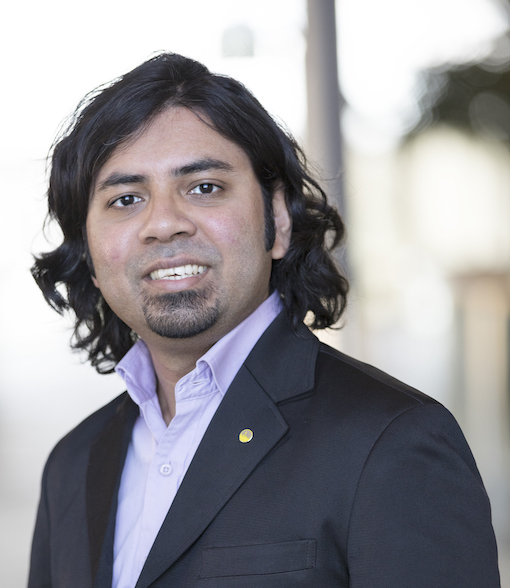
\includegraphics[scale=0.188, bottom]{photo.jpg}}}


%----------------------------------------------------------------------------------------
%	SIDEBAR SECTION
%----------------------------------------------------------------------------------------

\begin{aside} % In the aside, each new line forces a line break
~
Born on 27 September, 1986
~
\section{contact}
\vspace{5pt}\small{Risk and Environmental Studies
Department of Environmental and Life Sciences
Karlstad University
Universitetsgatan 2
SE 651 88 Karlstad, Sweden
~
Tel: +46 (0)54 700 10 44
Fax: +46 (0)54 700 10 44
~
E-mail: \href{mailto:avit.bhowmik@kau.se}{avit.bhowmik@kau.se}
Web: \href{http://avitbhowmik.ml/}{\small{http://avitbhowmik.ml/}}}
~
\section{research areas}
\vspace{5pt}Sustainability transformation
Climate
Risk Assessment
Environmental epidemiology
Remote Sensing
Geostatistics
GIS
~
\section{technical skills}
\vspace{5pt} \textbf{Programing \& Modelling}
R, C++, Python, Netlogo and Unix Shell'
%------------------------------------------------
\vspace{5pt}\textbf{Databases}
SQL and PostgreSQL
%------------------------------------------------
\vspace{5pt}\textbf{Geoinformatics}
GRASS GIS, Quantum GIS, ArcGIS, GeoMS, and ERDAS IMAGINE
%------------------------------------------------
\vspace{5pt}\textbf{Communication and Presentation}
HTML, CSS, MarkDown and \LaTeX
%------------------------------------------------
~
\section{languages}
\vspace{5pt}Bangla: mother tongue
English: level C2
German: level B2
Swedish: level A1
Portuguese: level A1

\vspace{10pt} \tiny{(Levels: A1/2: Basic user - B1/2: Independent user - C1/2: Proficient user, according to Common European Framework of Reference for Languages)}}

\end{aside}

%----------------------------------------------------------------------------------------
% KEY ACHIEVEMENTS SECTION
%----------------------------------------------------------------------------------------
\section{key achievements}

\begin{entrylist}
%------------------------------------------------
\entry
{\small{2018 - 2019}}
{\href{https://exponentialroadmap.org}{Exponential Climate Action Roadmap}} 
{}
{Have been leading the modelling exercises to lay out the first exponential pathways for climate action to halve greenhouse gas emission every decade from 2020 through 2050, the first output report from which was the highlight of \href{https://www.globalclimateactionsummit.org}{Global Climate Action Summit}, held in San Francisco, September 2018, and an update was released during the \href{https://www.un.org/en/climatechange/un-climate-summit-2019.shtml}{UN Climate Action Summit 2019}.}
%------------------------------------------------
\entry
{\small{2018}}
{\href{http://www.iiasa.ac.at/web/home/research/twi/TWI2050.html}{The World in 2050}} 
{}
{Contributed to shape the narrative and pathways for achieving the Sustainable Development Goals of the ``Agenda 2030'' in collaboration with a consortium of international scientists and policy makers, hosted in International Institue of Applied System Analysis (IIASA), the first output report of which was presented in \href{https://sustainabledevelopment.un.org/hlpf/2018}{United Nations High Level Political Forum}, July 2018.}
%------------------------------------------------
\entry
{\small{2017}}
{European Research Council (ERC) Advanced Grant} 
{}
{Co-applicant and contributed with drafting, reviewing and geospatial research expertise to a successful ERC Advanced grant proposal, i.e. ``Earth Resilience in the Anthropocene (ERA)'' (2,500,000 euro), Principal Investigator: Prof. Dr. Johan Rockström.}
%------------------------------------------------
\entry
{\small{2016}}
{Arctic Science Ministerial Report} 
{}
{Provided expert opinion for spatiotemporal variability modelling of climate and resilience in the Arctic, which shaped the policy framework of the ``U.S.-Canada Joint Statement on Climate, Energy, and Arctic Leadership'' in the first White House Arctic Science Ministerial Meeting on September 28, 2016.}
%------------------------------------------------
\entry
{\small{2015}}
{Novel Algorithm: ATRIC}
{}
{Developed the first open-source geospatial algorithm for automated stream threshold selection and riparian corridor delineation, which is currently being used by the ``Amazon Conservation Team'' in Columbia to assess deforestation impacts on the Amazon river. See \href{http://www.sciencedirect.com/science/article/pii/S1364815214003077}{here} for details.}
%------------------------------------------------

\end{entrylist}

%----------------------------------------------------------------------------------------
% EDUCATION SECTION
%----------------------------------------------------------------------------------------
%\newpage
\section{education}

\begin{entrylist}
%------------------------------------------------
\entry
{\small{09/2011--12/2015}}
{Doctor of Natural Sciences}
{University of Koblenz-Landau, Germany}
{Quantitative Landscape Ecology, Institute for Environmental Sciences\\
Dissertation: {\emph{Human and Ecological Impacts of Freshwater Degradation on Large Scales. Development and Integration of Spatial Models with Ecological Models for Spatial-ecological Analyses} (supervisor: Prof. Dr. Ralf B. Sch\"afer)} \\
Specialization: Spatial Statistics, Freshwater Eco(toxico)logy, Climate\\
Grade: 1.0 (top ranked) on a scale of 1.0 - 3.0 (1.0 best and 3.0 sufficient)}
%------------------------------------------------
\entry
{\small{09/2010--03/2012}}
{Master of Science {\normalfont{\footnotesize{in Geospatial Technologies}}}}
{Erasmus Mundus, European Commission}
{Partners: 1. School of Statistics and Information Management, New University of Lisbon, Portugal, 2. Institute for Geoinformatics (ifgi), University of M\"unster, Germany and 3. Department of Computer Languages and Systems, University of Jaume I, Spain}
\end{entrylist}
\section{}
\begin{entrylist}
\entry
{}
{}
{}
{Dissertation: {\emph{Evaluation of Spatial Interpolation Techniques for Mapping Climate Variables with low sample density. A case study using a new gridded dataset of Bangladesh} (supervisor: Prof. Dr. Ana Cristina Costa)} \\
Major: Geostatistics, Geographic Information Science (GIS), Climate \\
Grade: 18 (top ranked) on a scale of 1 - 20 (20 best and 1 worst)}
%------------------------------------------------
\entry
{\small{12/2004--10/2009}}
{Bachelor of Science {\normalfont{\scriptsize{in Urban \& Regional Planning}}}}
{\scriptsize{Bangladesh University of Engineering \& Technology}}
{Department of Urban \& Regional Planning\\
Dissertation: {\emph{Relocation of the Hazaribagh Tannery: Myth or Reality?} (supervisor: Prof. Dr. Md. Shakil Akther)}\\
Major: GIS, Environmental and Ecological Planning \\
Grade: 3.79 on a scale of 0-4.0 (4.0 best and 0 worst)}
%------------------------------------------------
\end{entrylist}

%----------------------------------------------------------------------------------------
%	WORK EXPERIENCE SECTION
%----------------------------------------------------------------------------------------
\section{professional appointments}

\begin{entrylist}
%------------------------------------------------
\entry
{\small{03/2019--present}}
{Assistant Professor}
{Karlstad University, Sweden}
{Risk and Environmental Studies, Department of Environmental and Life Sciences}
%------------------------------------------------
\entry
{\small{01/2018--02/2019}}
{Postdoctoral Researcher \& Liaison}
{Royal Swedish Academy of Sciences}
{Future Earth \\
1. \href{https://x-cac.futureearth.org/} {Exponential Climate Action} project: Backcasting modelling of climate action strategies to achieve Paris Agreement following the Carbon Law\\
2. \href{http://www.iiasa.ac.at/web/home/research/twi/TWI2050.html} {The World in 2050} project: Geospatial modelling and spatiotemporal analyses of drivers and processes underlying Sustainable Development Goals\\
3. Secretariat Liaison: Global Research Projects: (i) Analysis, Integration and Modelling of the Earth System (AIMES) and (ii) Integrated History and Future of People On Earth (IHOPE), and Knowledge Action Networks: (i) Decarbonization and (ii) Sustainable Development Goals}
%------------------------------------------------
\entry
{\small{01/2018--02/2019}}
{Guest Researcher}
{Stockholm University, Sweden}
{Stockholm Resilience Centre (Planetary Boundaries)}
%------------------------------------------------
\entry
{\small{01/2016--12/2017}}
{Postdoctoral Researcher}
{Stockholm University, Sweden}
{Stockholm Resilience Centre (Planetary Boundaries) \\
Cross-scale dynamics and spatial resilience patterns in social-ecological domains (led by Prof. Dr. Johan Rockstr\"om)}
%------------------------------------------------
\entry
{\small{01/2016--03/2018}}
{Guest Lecturer}
{University of Koblenz-Landau, Germany}
{Courses: 1. GIS Application, 2. GIS Projects for Advanced, 3. Introduction to open-source software and R for spatial ecotoxicological analyses, and 4. Spatial(-Temporal) Interpolation with R}
%------------------------------------------------
\entry
{\small{11/2015--12/2015}}
{Research Assistant}
{University of Koblenz-Landau, Germany}
{Quantitative Landscape Ecology, Institute for Environmental Sciences\\
Project - AufLand: Understanding effects of land use on the energy transfer across the freshwater-land interface}
%------------------------------------------------
\entry
{\small{04/2012--07/2012}}
{Research Assistant}
{University of M\"unster, Germany}
{Institute for Geoinformatics (ifgi)\\
Development of online demonstrators and web tools for core concepts of spatial information}
%------------------------------------------------
\end{entrylist}
\section{}
\begin{entrylist}
\entry
{\small{03/2008--10/2010}}
{Project Assistant}
{Technical University of Dortmund, Germany}
{{\emph{The Struggle for Urban Livelihoods and the Quest for a Functional City Reconciling Informal and Statutory Planning Institutions in Dhaka, Bangladesh,}} supported by the German Research Foundation (DFG) and conducted by the Department of Urban and Regional Planning, Faculty of Spatial Planning\\
Preparation of Geographic Information Systems (GIS) databases, analyses and processing of empirical data, conduction of empirical field investigation, i.e. key informant interviews, group discussion, household interviews and exercise of Venn-diagrams and observations}
%------------------------------------------------
\entry
{\small{10/2009--08/2010}}
{Assistant Town Planner}
{Concorde Land Development Limited, Dhaka, Bangladesh}
{Preparation of GIS databases, land use and subdivision plans}
%------------------------------------------------
\end{entrylist}

%----------------------------------------------------------------------------------------
% RESEARCH VISITS SECTION
%----------------------------------------------------------------------------------------
\section{research visits}

\begin{entrylist}
%------------------------------------------------
\entry
{\small{03/2018--04/2018}}
{Research Stay}
{International Institute for Applied Systems Analysis (IIASA)}
{Energy Program \\
Regional disparities among the trade-offs and co-benefits in the underlying processes of Sustainable Development Goals}
%------------------------------------------------
\end{entrylist}

%----------------------------------------------------------------------------------------
% PUBLICATIONS SECTION
%----------------------------------------------------------------------------------------
\section{publications}
\section{bibliographic metrics}

\begin{entrylist}
%------------------------------------------------
\entry
{\textbf{h-index: 12}}
{\hspace{10pt}i10-index: 15\hspace{35pt} 388 citations since 2012}
{source: {\href{https://scholar.google.de/citations?user=laRo5pgAAAAJ&hl=en}{google scholar}}}

\end{entrylist}

\vspace{-0.8cm}

\begin{refsection}
\nocite{*}
\printbibliography[type={article}, keyword={workpaper}, title={working papers}, heading=subbibliography]
\end{refsection}

\begin{refsection}
\nocite{*}
\printbibliography[type={article}, notkeyword={workpaper}, title={peer reviewed journal articles}, heading=subbibliography]
\end{refsection}
%\printbibsection{article}{peer reviewed journal articles} % Print all articles from the bibliography
\printbibsection{incollection}{book chapters} % Print all books from the bibliography
%\newpage
\printbibsection{report}{reports \& policy papers} % Print all reports from the bibliography
\begin{refsection}
\nocite{*}
\printbibliography[type={inproceedings}, keyword={confpaper}, title={conference papers}, heading=subbibliography]
\end{refsection}
%----------------------------------------------------------------------------------------
%----------------------------------------------------------------------------------------
% Presentation SECTION
%----------------------------------------------------------------------------------------

\section{presentations}
\begin{refsection}
\nocite{*}
\printbibliography[type={inproceedings}, keyword=invpres, title={invited presentations}, heading=subbibliography]
\end{refsection}

\begin{refsection}
\nocite{*}
\printbibliography[type={inproceedings}, keyword=presconf, title={conference presentations \& abstracts}, heading=subbibliography]
\end{refsection}

%------------------------------------------------

%----------------------------------------------------------------------------------------
% GRANT SECTION
%----------------------------------------------------------------------------------------
\section{research grants}

\begin{entrylist}
%------------------------------------------------
\entry
{\small{2018}}
{How to develop cross-scale and target seeking transformation scenarios through participatory processes?}
{PI: Dr. Avit K. Bhowmik}
{Bolin Centre for Climate Research\\
Total grant: 9,000 euro\\
Seed grant for pilot research projects on Sustainable Development Goals}
%------------------------------------------------
\end{entrylist}
\section{}
\begin{entrylist}
\entry
{\small{2016}}
{Earth Resilience in the Anthropocene (ERA)}
{Co-applicant, PI: Prof. Dr. Johan Rockström}
{European Research Council (ERC) Advanced Grant\\
Total grant: 2,500,000 euro\\
Contributions: (a) wrote and reviewed the grant proposal, (b) led work packages 2 \& 4, (c) added geospatial research expertise}
%------------------------------------------------
\entry
{\small{2017}}
{Social-ecological Resilience in the Anthropocene}
{PI: Dr. Avit K. Bhowmik}
{Department of Biology, Stockholm University\\
Total grant: 4,200 euro\\
Supported and supervised three master's theses projects}
%------------------------------------------------
\entry
{\small{2012--2015}}
{Quantitative Landscape Ecology Ph.D. Grant}
{PI: Avit K. Bhowmik}
{University of Koblenz-Landau, Germany\\
German Research Foundation (DFG) supported project\\
Total grant: 36,000 euro}
%------------------------------------------------
\entry
{\small{2010--2012}}
{Erasmus Mundus Scholarship}
{}
{{\emph{Master of Science in Geospatial Technology}} \\
The Education, Audiovisual and Culture Executive Agency (EACEA), European Commission\\
Total grant: 24,000 euro}
%------------------------------------------------
\end{entrylist}

%----------------------------------------------------------------------------------------
% Algorithm development SECTION
%----------------------------------------------------------------------------------------
\section{models \& software development}

\begin{entrylist}
%------------------------------------------------
\entry
{\small{10/2012}}
{ATRIC}
{}
{Automated Accumulation Threshold selection and RIparian Corridor delineation \\
Developed by co-interfacing R and GRASS GIS \\
Development page: \href{https://github.com/AvitBhowmik/ATRIC}{https://github.com/AvitBhowmik/ATRIC}}
%------------------------------------------------
\entry
{\small{08/2011}}
{SSTP}
{}
{Spatially Shifting Temporal Points \\
Developed using the gstat package utilities in R \\
Development page: \href{https://github.com/AvitBhowmik/SSTP}{https://github.com/AvitBhowmik/SSTP}}
%------------------------------------------------
\end{entrylist}

%----------------------------------------------------------------------------------------
% PROJECTS SECTION
%----------------------------------------------------------------------------------------
\section{research projects}

\begin{entrylist}
%------------------------------------------------
\entry
{\small{2016--present}}
{Environmentally triggered social collapse: Identifying confounding spatial drivers of demographic changes, armed conflicts and epidemic diseases}
{}
{Collaborator: The Earth League and University of Southampton, UK}
%------------------------------------------------
\entry
{\small{2016--2019}}
{Powers of 10: Scaling climate action strategies from individual to global
scales}
{}
{Collaborator: National University for Public Service, Budapest, Hungary and Project Drawdown}
%------------------------------------------------
\entry
{\small{2016--2019}}
{Social tipping elements instrumental for decarbonization by 2050}
{}
{Collaborators: The Earth League, Potsdam Institute for Climate Impact Research (PIK), Germany and Climate Service Center, Germany}
%------------------------------------------------
\entry
{\small{2017--2018}}
{The Great Acceleration Wave: Spatial propagation patterns of human driven natural resources exploitations}
{}
{Collaborator: Fenner School of Environment and Society, the Australian National University}
%----------------------------------------------------------------------------------------
\end{entrylist}
\section{}
\begin{entrylist}
\entry
{\small{2015--2017}}
{Effects of extreme climate events and landuse dynamics on the freshwater ecosystems in Europe}
{}
{Collaborator: Institute for Environmental Sciences, University of Koblenz-Landau, Germany}
%----------------------------------------------------------------------------------------
\entry
{\small{2014--present}}
{Human and ecological risks of freshwater and dust contaminations in developing countries}
{}
{Collaborators: COMSTATS Institute of Information and Technology, Pakistan and The Chinese Academy of Sciences}
%----------------------------------------------------------------------------------------
\entry
{\small{2012--2017}}
{Filling climate data-gaps: evaluation of the existing geostatistical methods and tools, and developing novel tools for improving climate spatial variability modelling in data-scarce regions}
{}
{Collaborators: New University of Lisbon, Portugal and The Chinese Academy of Sciences}
%----------------------------------------------------------------------------------------
\end{entrylist}

%----------------------------------------------------------------------------------------
% AWARDS SECTION
%----------------------------------------------------------------------------------------
\section{scholarships \& awards}
\begin{entrylist}
%------------------------------------------------
\entry
{\small{2014}}
{AGILE Early Career Scientist Grant}
{}
{17th International Conference on Geographic Information Science, Castellon, Spain}
%------------------------------------------------
\entry
{\small{2013}}
{CORDEX Young Scientist Award}
{}
{International Conference on Regional Climate - CORDEX 2013, Brussels, Belgium}
%------------------------------------------------
\entry
{\small{2013}}
{Best Paper Award}
{}
{{\emph{Space-Time Variability of Summer Temperature Field over Bangladesh during 1948-2007}} \\
13th International Conference on Computational Science and its Applications (ICCSA 2013), Ho Chi Minh City, Vietnam}
%------------------------------------------------
\entry
{\small{2009}}
{Mitsubishi Corporation International Merit Scholarship}
{}
{{\emph{For excellent academic performance in bachelor's studies}} \\
Mitsubishi Corporation, Japan}
%------------------------------------------------
\entry
{\small{2009}}
{University Grants Commission Merit Scholarship}
{}
{{\emph{For sound academic and extra-curricular activities}} \\
University Grants Commission of Bangladesh}
%------------------------------------------------
\end{entrylist}

%----------------------------------------------------------------------------------------
% Teaching Activities SECTION
%----------------------------------------------------------------------------------------
\section{teaching activities}

\begin{entrylist}
%------------------------------------------------
\entry
{\small{2019--present}}
{Nordic Climate Change Studies}
{}
{Risk and Environmental Studies, Karlstad University, Sweden}
%------------------------------------------------
\entry
{\small{2019--present}}
{Introduction Environment and Safety}
{}
{Risk and Environmental Studies, Karlstad University, Sweden}
%------------------------------------------------
\entry
{\small{2019--present}}
{Tools of environmental and safety management}
{}
{Risk and Environmental Studies, Karlstad University, Sweden}
%------------------------------------------------
\entry
{\small{2019--present}}
{The natural science basis of risk and environmental issues}
{}
{Risk and Environmental Studies, Karlstad University, Sweden}
%------------------------------------------------
\entry
{\small{2016--2018}}
{Use of Open Source Spatial Analysis Tools}
{}
{Online course on Spatial Ecotoxicology and Ecotoxicological Risk Assessment - Using an Open Community Approach, Institute for Environmental Sciences, University of Koblenz-Landau, Germany}
%------------------------------------------------
\end{entrylist}
\begin{entrylist}
\entry
{\small{2016--2018}}
{Entering the Anthropocene (Challenges of the Anthropocene)}
{}
{Course: Social-ecological Resilience for Sustainable Development, Stockholm Resilience Centre, Stockholm University, Sweden}
%------------------------------------------------
\entry
{\small{2015}}
{Spatial autocorrelation in ecological modelling}
{}
{Workshop 1: Data analysis in freshwater ecology using R, 9th Symposium for European Freshwater Sciences (SEFS), Geneva, Switzerland}
%------------------------------------------------
\entry
{\small{2013--2018}}
{Spatial(-Temporal) Interpolation with R}
{}
{International Summer Academy on Spatial Ecotoxicology and Ecotoxicological Risk Assessment-Using an Open Community Approach (funded by the German Academic Exchange Service (DAAD))}
%------------------------------------------------
\entry
{\small{2013--2018}}
{Introduction to open-source software and R for spatial ecotoxicological analyses}
{}
{International Summer Academy on Spatial Ecotoxicology and Ecotoxicological Risk Assessment-Using an Open Community Approach (funded by DAAD)}
%------------------------------------------------
\entry
{\small{2013--2018}}
{GIS Application with R}
{}
{Institute for Environmental Sciences, University of Koblenz-Landau, Germany}
%------------------------------------------------
\entry
{\small{2013--2018}}
{GIS Projects for Advanced}
{}
{Institute for Environmental Sciences, University of Koblenz-Landau, Germany}
%------------------------------------------------
\entry
{\small{2012}}
{Reference Systems for Geographic Information}
{}
{Institute for Geoinformatics, University of M\"unster, Germany}
%------------------------------------------------
\entry
{\small{2012}}
{Developing Demonstrators for Core Concepts of Spatial Information}
{}
{Institute for Geoinformatics, University of M\"unster, Germany}
%------------------------------------------------
\entry
{\small{2012}}
{Introduction to Digital Cartography}
{}
{Institute for Geoinformatics, University of M\"unster, Germany}
%------------------------------------------------
\end{entrylist}

%----------------------------------------------------------------------------------------
% Supervision SECTION
%----------------------------------------------------------------------------------------

\section{supervision}

\textbf{Doctoral Theses}

\begin{entrylist}
%------------------------------------------------
\entry
{\small{2016--2019}}
{A fusion remote sensing approach to the quantification of urban to global scale social-ecological impacts of anthropogenic land use and land cover changes}
{}
{R. Padmanaban, Doctoral dissertation \\
Nova Information Management School, New University of Lisbon, Portugal}
%------------------------------------------------
\entry
{\small{2016--present}}
{Land use and land cover change in Nigeria: A dynamic land system model approach}
{}
{A.O. Arowolo, Doctoral dissertation \\
Chinese Academy of Sciences, China and Federal University of Agriculture, Nigeria}
%------------------------------------------------
\end{entrylist}

\vspace{-0.3cm}
\textbf{Master's Theses}

\begin{entrylist}
%------------------------------------------------
\entry
{\small{2017--2018}}
{The Great Acceleration Wave: A timeline of human exploitation of the earth}
{}
{D. Fagerlind, Master's dissertation \\
Stockholm Resilience Centre, Stockholm University, Sweden}
%------------------------------------------------
\entry
{\small{2017--2018}}
{Transforming long distance travelling. A qualitative study of incentives to limit air travel in the face of climate change}
{}
{L. Jacobson, Master's dissertation \\
Stockholm Resilience Centre, Stockholm University, Sweden}
%------------------------------------------------
\entry
{\small{2016--2017}}
{‘Hazaribagh’- development trajectory or trap? A case study of a leather processing unit in Bangladesh}
{}
{F. Aktar, Master's dissertation \\
Stockholm Resilience Centre, Stockholm University, Sweden}
%------------------------------------------------
\end{entrylist}
\begin{entrylist}
\entry
{\small{2014--2016}}
{Effects of landuse on the energy transfer across the freshwater-land interface}
{}
{S. V. Kakarlapudi, Master's dissertation \\
Institute for Environmental Sciences, University of Koblenz-Landau, Germany}
%------------------------------------------------
\entry
{\small{2013--2015}}
{Extreme weather events and its effects on stream macroinvertebrates: Did the heat wave of 2003 cause a decline in the distribution of stream-macroinvertebrates in German low mountain ranges?}
{}
{G. Oehmichen, Diploma dissertation \\
Institute for Environmental Sciences, University of Koblenz-Landau, Germany}
%------------------------------------------------
\entry
{\small{2012--2013}}
{Mapping the ecological risk of agricultural pesticide runoff for Rheinland Palatinate}
{}
{L. Schneider, Master's dissertation \\
Institute for Environmental Sciences, University of Koblenz-Landau, Germany}
%------------------------------------------------
\end{entrylist}


\section{students' evaluation}

\begin{entrylist}
%------------------------------------------------
\entry
{}
{Overall Score: 1.25 - 2.0 on a scale from 1 to 5}
{1 best and 5 worst}
{}
%------------------------------------------------
\end{entrylist}

\section{pedagogical training}

\begin{entrylist}
%------------------------------------------------
\entry
{\small{2019}}
{Teaching in Higher Education}
{}
{Karlstad University Sweden}
%------------------------------------------------
\entry
{\small{January 2018}}
{Teachers' Conference 2018}
{Stockholm University Sweden}
{Being a university teacher in an ever-changing world}
%------------------------------------------------
\entry
{\small{October 2013}}
{Formal pedagogical training on university teaching}
{}
{Higher Education Teaching Center, University of Koblenz-Landau, Germany}
%------------------------------------------------
\end{entrylist}

%----------------------------------------------------------------------------------------
% NETWORKS
%----------------------------------------------------------------------------------------
\section{science-policy-industry networks}

\begin{entrylist}
%------------------------------------------------
\entry
{\small{2016--2019}}
{Earth-Doc, \href{http://www.the-earth-league.org/earth-doc-bios.html}{The Earth League}}
{}
{Project: Earth Lander - Social tipping elements instrumental for decarbonization by 2050}
%------------------------------------------------
\entry
{\small{2016--2018}}
{Analysis, Integration and Modelling of the Earth System (AIMES)}
{}
{Associated with the international project office in Sweden}
%----------------------------------------------------------------------------------------
\entry
{\small{2016--2018}}
{European Space Agency}
{}
{Project: \href{http://earthsystemdatacube.net/}{Earth System Data Cube}, partners: Brockmann Consultant Gmbh, Max Planck Institute for Biogeochemistry and Stockholm Resilience Centre}
%------------------------------------------------
\entry
{\small{2018--2019}}
{Future Earth}
{}
{Liaised with and coordinating two Global Research Projects and two Knowledge Action Networks}
%----------------------------------------------------------------------------------------
\entry
{\small{2016--present}}
{Sustainable Development Solutions Network (SDSN)}
{}
{Project: The World in 2050 (TWI 2050)}
%----------------------------------------------------------------------------------------
\entry
{\small{2015--2018}}
{European Geosciences Union (EGU)}
{}
{Member}
%----------------------------------------------------------------------------------------
\entry
{\small{2013--present}}
{Society of Ecotoxicology and Chemistry (SETAC)}
{}
{Member}
%----------------------------------------------------------------------------------------
\end{entrylist}

%----------------------------------------------------------------------------------------
% EDITORIAL SECTION
%----------------------------------------------------------------------------------------
\newpage
\section{editorial activities}

\begin{entrylist}
%------------------------------------------------
\entry
{\small{2018--2019}}
{Guest Editor}
{}
{Sustainability Science}
%------------------------------------------------
\entry
{\small{2016--2019}}
{Reviewer for research project grants}
{}
{Future Earth Sustainable Development Goals Labs\\
Chilean National Science and Technology Commission}
%------------------------------------------------
\entry
{\small{2016--present}}
{Editorial board member}
{}
{Water Science and Technology: Water Supply}
%------------------------------------------------
\entry
{\small{2014--present}}
{Ad-hoc reviewer}
{}
{Global Ecology and Biogeography\\
Ecography\\
International Journal of Climatology\\
Sustainability\\
PLOS ONE\\
Earth Science Informatics\\
Geomatics, Natural Hazards and Risk\\
Journal of Environmental Informatics\\
Applied Ecology and Environmental Research\\
Journal of Health and Pollution\\
Natural Hazards\\
Geosciences\\
Geoscience Data Journal\\
Environmental Monitoring and Assessment\\
International Journal of Environmental Research and Public Health\\
Agronomy\\
Geomorphology}

\end{entrylist}

%----------------------------------------------------------------------------------------
% Leadership Skills SECTION
%----------------------------------------------------------------------------------------
\section{leadership, management \& administration}

\begin{entrylist}
%------------------------------------------------
\entry
{\small{04/2018}}
{Principal Organizer}
{}
{Workshop: Exponential Climate Action for Cities, Carbon Law Accelerator project, Future Earth, Stockholm, Sweden}
%------------------------------------------------
\entry
{\small{02/2018}}
{Theme Leader}
{}
{Pathways to new collaborations in climate research at Stockholm University: Perspectives from the Human Science Academic Area and the Bolin Centre for Climate Research}
%------------------------------------------------
\entry
{\small{08/2017}}
{Session Chair}
{}
{Session: Exploring the potential of local innovations and bottom-up change, Social-ecological transformations for sustainability, Resilience 2017 - Resilience Frontiers for Global Sustainability}
%------------------------------------------------
\entry
{\small{06/2017}}
{Principal Organizer}
{}
{Workshop: Progress in computational macroecology, The 17th International Conference on Computational Science and Its Applications (ICCSA 2017), Trieste, Italy}
%------------------------------------------------
\entry
{\small{12/2016}}
{Principal Organizer}
{}
{Social Tipping Elements Instrumental for Decarbonization by 2050: an Expert Workshop, The Earth League, Stockholm Resilience Centre, Sweden}
%------------------------------------------------
\end{entrylist}
\section{}
\begin{entrylist}
\entry
{\small{09/2016}}
{Co-organizer}
{}
{Climate Tipping Points and Safe Pathways to Sustainable Development: an expert review workshop, Stockholm Resilience Centre, Stockholm, Sweden\\
Analysis, Integration and Modelling of the Earth System (AIMES)}
%------------------------------------------------
\entry
{\small{05/2016}}
{Principal Organizer}
{}
{3rd Earth-Doc Meeting, Stockholm Resilience Centre, Sweden\\
(a) Preparation of a strategy document outlining Earth-Doc research, and (b) Advancing on the on-going Earth-League research proposal and perspective paper}
%------------------------------------------------
\entry
{\small{07/2015}}
{Principal Organizer}
{}
{Workshop 1: Data analysis in freshwater ecology using R, 9th Symposium for European Freshwater Sciences (SEFS), Geneva, Switzerland}
%------------------------------------------------
\entry
{\small{09/2012--12/2015}}
{Developer and Maintainer}
{}
{Geodata Server \\ 
Institute for Environmental Sciences, University of Koblenz-Landau, Germany}
%------------------------------------------------
\entry
{\small{11/2010--02/2011}}
{Group Leader}
{}
{Spatial statistics group \\ 
Group project seminar on Identifying optimal location for disaster evacuation centres in Lisbon, New University of Lisbon, Portugal}
%------------------------------------------------
\entry
{\small{07/2007--present}}
{U.S. Department of State Alumni}
{}
{Study of the United States Institute for Student Leaders 2007, organized by the United States Department of State in Washington and Green River Community College, Seattle, USA\\
Community services}
%------------------------------------------------
\end{entrylist}

%----------------------------------------------------------------------------------------
% WORKSHOP AND TRAINING SECTION
%----------------------------------------------------------------------------------------
\section{workshops \& trainings}

\begin{entrylist}
%------------------------------------------------
\entry
{\small{April 2013}}
{Final Colloquium of the priority program "Megacities-Megachallenge: Informal Dynamics of GlobalChange"}
{}
{German Research Foundation (DFG), Bonn, Germany}
%------------------------------------------------
\entry
{\small{January 2013}}
{Mechanistic Effect Modelling for Ecological Risk Assessment of Chemicals}
{}
{Society of Environmental Toxicology and Chemistry (SETAC) and Helmholtz Centre for Environmental Research - UFZ, Leipzig, Germany}
%------------------------------------------------
\entry
{\small{February 2012}}
{Recent Development in Geostatistics: Change of Support and Spatial Analysis of Temporal Trends in Health Outcomes}
{}
{Dr. Pierre Goovaerts (Computer Sciences Corporation), School of Statistics and Information Management, New University of Lisbon, Portugal}
%------------------------------------------------
\end{entrylist}

\newline
\vspace{2cm}
\normalfont{Karlstad, \today}}
\newline
\newline

\includegraphics[width=0.2\linewidth]{signature.png}
\newline
\textbf{Avit K. Bhowmik}
%----------------------------------------------------------------------------------------

\end{document}